	\documentclass[11pt]{article}
	
	\title{Homework 1 - DM CS6220}
	\author{Nakul Camasamudram}
	\usepackage{amsmath,amsfonts,amsthm} % Math packages
	\usepackage{mathtools}
	\usepackage{adjustbox}
	\usepackage{soul}
	\usepackage{enumitem}
	
	%----------------------------------------------------------------------------------------
	%	TITLE SECTION
	%----------------------------------------------------------------------------------------
	
	\newcommand{\horrule}[1]{\rule{\linewidth}{#1}} 
	
	\title{	
	\normalfont \normalsize 
	\textsc{Northeastern University, Data Mining Techniques - CS6220 Fall 2017} \\
	 % Your university, school and/or department name(s)
	\horrule{0.5pt} \\[0.4cm] % Thin top horizontal rule
	\huge Solutions to Homework 2, Part 2 \\ % The assignment title
	\horrule{2pt} \\[0.5cm] % Thick bottom horizontal rule
	}
	\author{Nakul Camasamudram} % Your name
	\date{\normalsize\today} % Today's date or a custom date
	\begin{document}
	
	\maketitle % Print the title
	\newpage
	
	%----------------------------------------------------------------------------------------
	%	PROBLEM 1
	%----------------------------------------------------------------------------------------
	
	\section*{1. K-Means}

	\textbf{Solution:}\\
    
    \begin{itemize}
    	\item \textbf{Iteration 1:} \\
    	The initial centroids are $C_1$ = (2, 10) $C_2$ = (1, 2) $C_3$ = (5, 8). Let D($C_i$) represent the \textbf{euclidean} distance between the respective point and the $i^{th}$ centroid.
    	
		\underline{The $E$-step:} \\
    		\begin{center}
    			\begin{adjustbox}{max width=\textwidth}
				\begin{tabular}{ | c | c | c | c | c |}
	  	 		\hline
    				\textbf{Data Point} & \textbf{D($C_1$)} & \textbf{D($C_2$)} & \textbf{D($C_3$)} & \textbf{Optimal centroid} \\ 
    			\hline
    				(4,9) & 2.23606797749979 & 7.615773105863909 & \textbf{1.4142135623730951} & $C_3$ \\ 
    			\hline
    				(2,10) & \textbf{0.0} & 8.06225774829855 & 3.605551275463989 & $C_1$ \\ 
    			\hline
					(1,2) & 8.06225774829855 & \textbf{0.0} & 7.211102550927978 & $C_2$ \\ 
    			\hline   
    				(2,5) & 5.0 & \textbf{3.1622776601683795} & 4.242640687119285 & $C_2$ \\ 
    			\hline
	    			(6,4) & 7.211102550927978 & 5.385164807134504 & \textbf{4.123105625617661} & $C_3$ \\ 
    			\hline
    				(8,4) & 8.48528137423857 & 7.280109889280518 & \textbf{5.0} & $C_3$ \\ 
    			\hline
    				(7, 5) & 7.0710678118654755 & 6.708203932499369 & \textbf{3.605551275463989} & $C_3$ \\ 
    			\hline 	
    				(5, 8) & 3.605551275463989 & 7.211102550927978 & \textbf{0.0} & $C_3$ \\ 
    			\hline 					
    			\end{tabular}
    			\end{adjustbox}
			\end{center}
		
		\underline{The $M$-step:} \\
		$C_1$ = mean[(2, 10)] = (2.0, 10.0) \\
		$C_2$ = mean[(1, 2), (2, 5)] = (1.5, 3.5) \\
		$C_3$ = mean[(4, 9), (6, 4), (8, 4), (7, 5), (5, 8)] = (6.0, 6.0) \\
		
		\begin{center}
			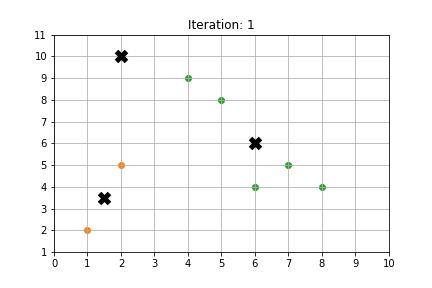
\includegraphics[scale=0.7]{kmeans_graphs/iteration_1.png}
		\end{center}

    	\item \textbf{Iteration 2:} \\
		\begin{center}
			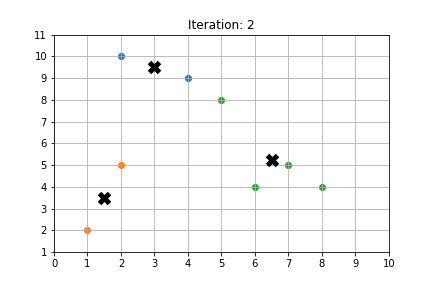
\includegraphics[scale=0.7]{kmeans_graphs/iteration_2.png}
		\end{center}
		
		\item \textbf{Iteration 3:} \\
		\begin{center}
			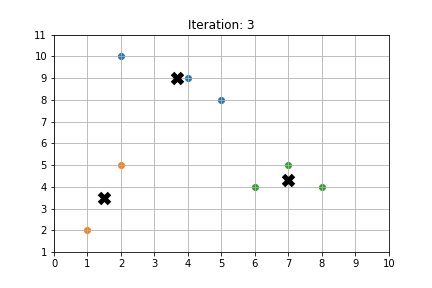
\includegraphics[scale=0.7]{kmeans_graphs/iteration_3.png}
		\end{center}
		
		\item \textbf{Iteration 4:} \\
		\begin{center}
			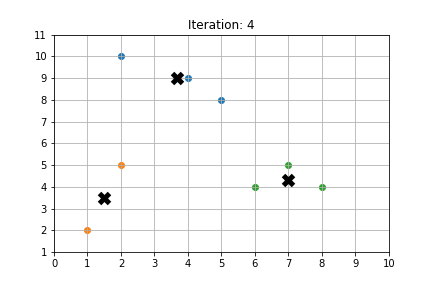
\includegraphics[scale=0.7]{kmeans_graphs/iteration_4.png}
		\end{center}
    \end{itemize}
	\newpage
	
	%----------------------------------------------------------------------------------------
	%	PROBLEM 2
	%----------------------------------------------------------------------------------------
	\section*{2. Agglomerative Hierarchical}

	\textbf{Solution:}\\
	
	\textbf{1. Using MIN as an inter-cluster measure} \\
	
	\textbf{Iteration 1:}
	
	\begin{center}
    	\begin{adjustbox}{max width=\textwidth}
		\begin{tabular}{ | c | c | c | c | c | c | c |}
	  	 	\hline

	  	 	& \textbf{$p_1$} & \textbf{$p_2$} & \textbf{$p_3$} & \textbf{$p_4$} & \textbf{$p_5$} & \textbf{$p_6$}\\
	  	 	\hline
	  	 	
	  	 	\textbf{$p_1$} &  &  &  &  &  &\\
	  	 	\hline
	  	 	
	  	 	\textbf{$p_2$} & 0.2421 &  &  &  &  &  \\
	  	 	\hline
	  	 	
	  	 	\textbf{$p_3$} & 0.2159 & 0.1523 &  &  &  & \\
	  	 	\hline
	  	 	
	  	 	\textbf{$p_4$} & 0.3677 & 0.1965 & 0.1581 &  &  & \\
	  	 	\hline
	  	 	
	  	 	\textbf{$p_5$} & 0.3418 & 0.1334 & 0.2846 & 0.2842 &  & \\
	  	 	\hline	
	  	 	
	  	 	\textbf{$p_6$} & 0.2354 & 0.2530 & \textbf{0.1020} & 0.2195 & 0.3860 & \\
	  	 	\hline			
    		\end{tabular}
    	\end{adjustbox}
	\end{center}
	
	\underline{Cluster 1:} \{3, 6\}
	
	\begin{itemize}
		\item d(\{1\},\{3,6\}) = min(d(\{1\},\{3\}), d(\{1\},\{6\})) = d(\{1\},\{3\})
		\item d(\{2\},\{3,6\}) = min(d(\{2\},\{3\}), d(\{2\},\{6\})) = d(\{2\},\{3\})
		\item d(\{4\},\{3,6\}) = min(d(\{4\},\{3\}), d(\{4\},\{6\})) = d(\{4\},\{3\})
		\item d(\{5\},\{3,6\}) = min(d(\{5\},\{3\}), d(\{5\},\{6\})) = d(\{5\},\{3\})
	\end{itemize}
	
	\vspace{5mm}
	
	\textbf{Iteration 2:}
	
	\begin{center}
    	\begin{adjustbox}{max width=\textwidth}
		\begin{tabular}{ | c | c | c | c | c | c | c |}
	  	 	\hline

	  	 	& \textbf{$p_1$} & \textbf{$p_2$} & \textbf{$p_3$} & \textbf{$p_4$} & \textbf{$p_5$} & \textbf{$p_6$}\\
	  	 	\hline
	  	 	
	  	 	\textbf{$p_1$} &  &  &  &  &  &\\
	  	 	\hline
	  	 	
	  	 	\textbf{$p_2$} & 0.2421 &  &  &  &  &  \\
	  	 	\hline
	  	 	
	  	 	\textbf{$p_3$} & 0.2159 & 0.1523 &  &  &  & \\
	  	 	\hline
	  	 	
	  	 	\textbf{$p_4$} & 0.3677 & 0.1965 & 0.1581 &  &  & \\
	  	 	\hline
	  	 	
	  	 	\textbf{$p_5$} & 0.3418 & \textbf{0.1334} & 0.2846 & 0.2842 &  & \\
	  	 	\hline	
	  	 	
	  	 	\textbf{$p_6$} & \st{0.2354} & \st{0.2530} & \st{0.1020} & \st{0.2195} & \st{0.3860} & \\
	  	 	\hline			
    		\end{tabular}
    	\end{adjustbox}
	\end{center}
	
	\underline{Cluster 1:} \{3, 6\} \\
	\underline{Cluster 2:} \{2, 5\}
	
	\begin{itemize}
		\item d(\{1\},\{2,5\}) = min(d(\{1\},\{2\}), d(\{1\},\{5\})) = d(\{1\},\{2\})
		\item d(\{4\},\{2,5\}) = min(d(\{4\},\{2\}), d(\{4\},\{5\})) = d(\{4\},\{2\})
		\item d(\{3,6\},\{2,5\}) = min(d(\{3\},\{2\}), d(\{3\},\{5\}), d(\{6\},\{2\}), d(\{6\},\{5\})) = d(\{3\},\{2\})
	\end{itemize}
	
	
	\vspace{5mm}
	
	
	\textbf{Iteration 3:}
	
	\begin{center}
    	\begin{adjustbox}{max width=\textwidth}
		\begin{tabular}{ | c | c | c | c | c | c | c |}
	  	 	\hline

	  	 	& \textbf{$p_1$} & \textbf{$p_2$} & \textbf{$p_3$} & \textbf{$p_4$} & \textbf{$p_5$} & \textbf{$p_6$}\\
	  	 	\hline
	  	 	
	  	 	\textbf{$p_1$} &  &  &  &  &  &\\
	  	 	\hline
	  	 	
	  	 	\textbf{$p_2$} & 0.2421 &  &  &  &  &  \\
	  	 	\hline
	  	 	
	  	 	\textbf{$p_3$} & 0.2159 & \textbf{0.1523} &  &  &  & \\
	  	 	\hline
	  	 	
	  	 	\textbf{$p_4$} & 0.3677 & 0.1965 & 0.1581 &  &  & \\
	  	 	\hline
	  	 	
	  	 	\textbf{$p_5$} & \st{0.3418} & \st{0.1334} & \st{0.2846} & \st{0.2842} &  & \\
	  	 	\hline	
	  	 	
	  	 	\textbf{$p_6$} & \st{0.2354} & \st{0.2530} & \st{0.1020} & \st{0.2195} & \st{0.3860} & \\
	  	 	\hline			
    		\end{tabular}
    	\end{adjustbox}
	\end{center}
	
	\underline{Cluster 1:} \{3, 6\} \\
	\underline{Cluster 2:} \{2, 5\} \\
	\underline{Cluster 3:} \{\{2, 5\}, \{3, 6\}\} 
	
	\begin{itemize}
		\item d\{\{2, 5, 3, 6\}, \{1\}\} = min(d\{2, 1\}, d\{5, 1\}, d\{3, 1\}, d\{6, 1\}) = d\{3, 1\}
		\item d\{\{2, 5, 3, 6\}, \{4\}\} = min(d\{2, 4\}, d\{5, 4\}, d\{3, 4\}, d\{6, 4\}) = d\{3, 4\}
	\end{itemize}
	
	
	\vspace{5mm}
	
	\textbf{Iteration 4:}
	
	\begin{center}
    	\begin{adjustbox}{max width=\textwidth}
		\begin{tabular}{ | c | c | c | c | c | c | c |}
	  	 	\hline

	  	 	& \textbf{$p_1$} & \textbf{$p_2$} & \textbf{$p_3$} & \textbf{$p_4$} & \textbf{$p_5$} & \textbf{$p_6$}\\
	  	 	\hline
	  	 	
	  	 	\textbf{$p_1$} &  &  &  &  &  &\\
	  	 	\hline
	  	 	
	  	 	\textbf{$p_2$} & \st{0.2421} &  &  &  &  &  \\
	  	 	\hline
	  	 	
	  	 	\textbf{$p_3$} & 0.2159 & \st{0.1523} &  &  &  & \\
	  	 	\hline
	  	 	
	  	 	\textbf{$p_4$} & 0.3677 & \st{0.1965} & \textbf{0.1581} &  &  & \\
	  	 	\hline
	  	 	
	  	 	\textbf{$p_5$} & \st{0.3418} & \st{0.1334} & \st{0.2846} & \st{0.2842} &  & \\
	  	 	\hline	
	  	 	
	  	 	\textbf{$p_6$} & \st{0.2354} & \st{0.2530} & \st{0.1020} & \st{0.2195} & \st{0.3860} & \\
	  	 	\hline			
    		\end{tabular}
    	\end{adjustbox}
	\end{center}
	
	\underline{Cluster 1:} \{3, 6\} \\
	\underline{Cluster 2:} \{2, 5\} \\
	\underline{Cluster 3:} \{\{2, 5\}, \{3, 6\}\} \\
	\underline{Cluster 4:} \{\{2, 5, 3, 6\}, \{4\}\}
	\newpage
	
	
	% ------
	
	\textbf{2. Using MAX as an inter-cluster measure} \\
	
	\textbf{Iteration 1:}
	
	\begin{center}
    	\begin{adjustbox}{max width=\textwidth}
		\begin{tabular}{ | c | c | c | c | c | c | c |}
	  	 	\hline

	  	 	& \textbf{$p_1$} & \textbf{$p_2$} & \textbf{$p_3$} & \textbf{$p_4$} & \textbf{$p_5$} & \textbf{$p_6$}\\
	  	 	\hline
	  	 	
	  	 	\textbf{$p_1$} &  &  &  &  &  &\\
	  	 	\hline
	  	 	
	  	 	\textbf{$p_2$} & 0.2421 &  &  &  &  &  \\
	  	 	\hline
	  	 	
	  	 	\textbf{$p_3$} & 0.2159 & 0.1523 &  &  &  & \\
	  	 	\hline
	  	 	
	  	 	\textbf{$p_4$} & 0.3677 & 0.1965 & 0.1581 &  &  & \\
	  	 	\hline
	  	 	
	  	 	\textbf{$p_5$} & 0.3418 & 0.1334 & 0.2846 & 0.2842 &  & \\
	  	 	\hline	
	  	 	
	  	 	\textbf{$p_6$} & 0.2354 & 0.2530 & \textbf{0.1020} & 0.2195 & 0.3860 & \\
	  	 	\hline			
    		\end{tabular}
    	\end{adjustbox}
	\end{center}
	
	\underline{Cluster 1:} \{3, 6\}
	
	\begin{itemize}
		\item d(\{1\},\{3,6\}) = max(d(\{1\},\{3\}), d(\{1\},\{6\})) = d(\{1\},\{6\})
		\item d(\{2\},\{3,6\}) = max(d(\{2\},\{3\}), d(\{2\},\{6\})) = d(\{2\},\{6\})
		\item d(\{4\},\{3,6\}) = max(d(\{4\},\{3\}), d(\{4\},\{6\})) = d(\{4\},\{6\})
		\item d(\{5\},\{3,6\}) = max(d(\{5\},\{3\}), d(\{5\},\{6\})) = d(\{5\},\{6\})
	\end{itemize}
	
	\vspace{5mm}
	
	\textbf{Iteration 2:}
	
	\begin{center}
    	\begin{adjustbox}{max width=\textwidth}
		\begin{tabular}{ | c | c | c | c | c | c | c |}
	  	 	\hline

	  	 	& \textbf{$p_1$} & \textbf{$p_2$} & \textbf{$p_3$} & \textbf{$p_4$} & \textbf{$p_5$} & \textbf{$p_6$}\\
	  	 	\hline
	  	 	
	  	 	\textbf{$p_1$} &  &  &  &  &  &\\
	  	 	\hline
	  	 	
	  	 	\textbf{$p_2$} & 0.2421 &  &  &  &  &  \\
	  	 	\hline
	  	 	
	  	 	\textbf{$p_3$} & \st{0.2159} & \st{0.1523} &  &  &  & \\
	  	 	\hline
	  	 	
	  	 	\textbf{$p_4$} & 0.3677 & 0.1965 & \st{0.1581} &  &  & \\
	  	 	\hline
	  	 	
	  	 	\textbf{$p_5$} & 0.3418 & \textbf{0.1334} & \st{0.2846} & 0.2842 &  & \\
	  	 	\hline	
	  	 	
	  	 	\textbf{$p_6$} & 0.2354 & 0.2530 & \st{0.1020} & 0.2195 & 0.3860 & \\
	  	 	\hline			
    		\end{tabular}
    	\end{adjustbox}
	\end{center}
	
	\underline{Cluster 1:} \{3, 6\} \\
	\underline{Cluster 2:} \{2, 5\}
	
	\begin{itemize}
		\item d(\{1\},\{2,5\}) = max(d(\{1\},\{2\}), d(\{1\},\{5\})) = d(\{1\},\{5\})
		\item d(\{4\},\{2,5\}) = max(d(\{4\},\{2\}), d(\{4\},\{5\})) = d(\{4\},\{5\})
		\item d(\{3, 6\},\{2,5\}) = max(d(\{3\},\{2\}), d(\{3\},\{5\}), d(\{6\},\{2\}), d(\{6\},\{5\})) = d(\{6\},\{5\})
	\end{itemize}
	
	\vspace{5mm}
	
	\textbf{Iteration 3:}
	
	\begin{center}
    	\begin{adjustbox}{max width=\textwidth}
		\begin{tabular}{ | c | c | c | c | c | c | c |}
	  	 	\hline

	  	 	& \textbf{$p_1$} & \textbf{$p_2$} & \textbf{$p_3$} & \textbf{$p_4$} & \textbf{$p_5$} & \textbf{$p_6$}\\
	  	 	\hline
	  	 	
	  	 	\textbf{$p_1$} &  &  &  &  &  &\\
	  	 	\hline
	  	 	
	  	 	\textbf{$p_2$} & \st{0.2421} &  &  &  &  &  \\
	  	 	\hline
	  	 	
	  	 	\textbf{$p_3$} & \st{0.2159} & \st{0.1523} &  &  &  & \\
	  	 	\hline
	  	 	
	  	 	\textbf{$p_4$} & 0.3677 & \st{0.1965} & \st{0.1581} &  &  & \\
	  	 	\hline
	  	 	
	  	 	\textbf{$p_5$} & 0.3418 & \st{0.1334} & \st{0.2846} & 0.2842 &  & \\
	  	 	\hline	
	  	 	
	  	 	\textbf{$p_6$} & 0.2354 & \st{0.2530} & \st{0.1020} & \textbf{0.2195} & 0.3860 & \\
	  	 	\hline			
    		\end{tabular}
    	\end{adjustbox}
	\end{center}
	
	\underline{Cluster 1:} \{3, 6\} \\
	\underline{Cluster 2:} \{2, 5\} \\
	\underline{Cluster 3:} \{\{3, 6\}, \{4\}\}
	
	\begin{itemize}
		\item d(\{1\},\{3,4,6\}) = max(d(\{1\},\{3\}), d(\{1\},\{4\}), d(\{1\},\{6\})) = d(\{1\},\{4\})
		\item d(\{2,5\},\{3,4,6\}) = max(d(\{2\},\{3\}), d(\{2\},\{4\}), d(\{2\},\{6\}), d(\{5\},\{3\}), d(\{5\},\{4\}), d(\{5\},\{6\})) = d(\{5\},\{6\})
	\end{itemize}
	
	\vspace{5mm}
	
	\textbf{Iteration 4:}
	
	\begin{center}
    	\begin{adjustbox}{max width=\textwidth}
		\begin{tabular}{ | c | c | c | c | c | c | c |}
	  	 	\hline

	  	 	& \textbf{$p_1$} & \textbf{$p_2$} & \textbf{$p_3$} & \textbf{$p_4$} & \textbf{$p_5$} & \textbf{$p_6$}\\
	  	 	\hline
	  	 	
	  	 	\textbf{$p_1$} &  &  &  &  &  &\\
	  	 	\hline
	  	 	
	  	 	\textbf{$p_2$} & \st{0.2421} &  &  &  &  &  \\
	  	 	\hline
	  	 	
	  	 	\textbf{$p_3$} & \st{0.2159} & \st{0.1523} &  &  &  & \\
	  	 	\hline
	  	 	
	  	 	\textbf{$p_4$} & 0.3677 & \st{0.1965} & \st{0.1581} &  &  & \\
	  	 	\hline
	  	 	
	  	 	\textbf{$p_5$} & \textbf{0.3418} & \st{0.1334} & \st{0.2846} & \st{0.2842} &  & \\
	  	 	\hline	
	  	 	
	  	 	\textbf{$p_6$} & \st{0.2354} & \st{0.2530} & \st{0.1020} & \st{0.2195} & 0.3860 & \\
	  	 	\hline			
    		\end{tabular}
    	\end{adjustbox}
	\end{center}
	
	\underline{Cluster 1:} \{3, 6\} \\
	\underline{Cluster 2:} \{2, 5\} \\
	\underline{Cluster 3:} \{\{3, 6\}, \{4\}\} \\
	\underline{Cluster 4:} \{\{2, 5\}, \{1\}\}
	\newpage
	
	% --------
	
	\textbf{1. Using AVG as an inter-cluster measure} \\
	
	\textbf{Iteration 1:}
	
	\begin{center}
    	\begin{adjustbox}{max width=\textwidth}
		\begin{tabular}{ | c | c | c | c | c | c | c |}
	  	 	\hline

	  	 	& \textbf{$p_1$} & \textbf{$p_2$} & \textbf{$p_3$} & \textbf{$p_4$} & \textbf{$p_5$} & \textbf{$p_6$}\\
	  	 	\hline
	  	 	
	  	 	\textbf{$p_1$} &  &  &  &  &  &\\
	  	 	\hline
	  	 	
	  	 	\textbf{$p_2$} & 0.2421 &  &  &  &  &  \\
	  	 	\hline
	  	 	
	  	 	\textbf{$p_3$} & 0.2159 & 0.1523 &  &  &  & \\
	  	 	\hline
	  	 	
	  	 	\textbf{$p_4$} & 0.3677 & 0.1965 & 0.1581 &  &  & \\
	  	 	\hline
	  	 	
	  	 	\textbf{$p_5$} & 0.3418 & 0.1334 & 0.2846 & 0.2842 &  & \\
	  	 	\hline	
	  	 	
	  	 	\textbf{$p_6$} & 0.2354 & 0.2530 & \textbf{0.1020} & 0.2195 & 0.3860 & \\
	  	 	\hline			
    		\end{tabular}
    	\end{adjustbox}
	\end{center}
	
	\underline{Cluster 1:} \{3, 6\}
	
	\begin{itemize}
		\item d(\{1\},\{3,6\}) = avg[d(\{1\},\{3\}) + d(\{1\},\{6\})] = 0.2256
		\item d(\{4\},\{3,6\}) = avg[d(\{4\},\{3\}) + d(\{4\},\{6\})] = 0.1888
		\item d(\{2\},\{3,6\}) = avg[d(\{2\},\{3\}) + d(\{2\},\{6\})] = 0.2026
		\item d(\{5\},\{3,6\}) = avg[d(\{5\},\{3\}) + d(\{5\},\{6\})] = 0.3353
	\end{itemize}
	
	\vspace{5mm}
	
	\textbf{Iteration 2:}
	
	\begin{center}
    	\begin{adjustbox}{max width=\textwidth}
		\begin{tabular}{ | c | c | c | c | c | c |}
	  	 	\hline

	  	 	& \textbf{$p_1$} & \textbf{$p_2$} & \textbf{$p_3, p_6$} & \textbf{$p_4$} & \textbf{$p_5$}\\
	  	 	\hline
	  	 	
	  	 	\textbf{$p_1$} &  &  &  &  &\\
	  	 	\hline
	  	 	
	  	 	\textbf{$p_2$} & 0.2421 &  &  &  &\\
	  	 	\hline
	  	 	
	  	 	\textbf{$p_3, p_6$} & 0.2256 & 0.2026 &  &  &\\
	  	 	\hline
	  	 	
	  	 	\textbf{$p_4$} & 0.3677 & 0.1965 & 0.1888 &  &\\
	  	 	\hline
	  	 	
	  	 	\textbf{$p_5$} & 0.3418 & \textbf{0.1334} & 0.3353 & 0.2842 &\\
	  	 	\hline			
    		\end{tabular}
    	\end{adjustbox}
	\end{center}
	
	\underline{Cluster 1:} \{3, 6\} \\
	\underline{Cluster 1:} \{2, 5\} \\
	
	\begin{itemize}
		\item d(\{1\},\{2,5\}) = avg[d(\{1\},\{2\}) + d(\{1\},\{5\})] = 0.2919
		\item d(\{3,6\},\{2,5\}) = avg[d(\{3,6\},\{2\}) + d(\{3,6\},\{5\})] = 0.2837
		\item d(\{4\},\{2,5\}) = avg[d(\{4\},\{2\}) + d(\{4\},\{5\})] = 0.2404
	\end{itemize}

	\vspace{5mm}
	
	\textbf{Iteration 3:}
	
	\begin{center}
    	\begin{adjustbox}{max width=\textwidth}
		\begin{tabular}{ | c | c | c | c | c |}
	  	 	\hline

	  	 	& \textbf{$p_1$} & \textbf{$p_2, p_5$} & \textbf{$p_3, p_6$} & \textbf{$p_4$}\\
	  	 	\hline
	  	 	
	  	 	\textbf{$p_1$} &  &  &  &\\
	  	 	\hline
	  	 	
	  	 	\textbf{$p_2, p_5$} & 0.2919 &  &  &\\
	  	 	\hline
	  	 	
	  	 	\textbf{$p_3, p_6$} & 0.2256 & 0.2185 &  &\\
	  	 	\hline
	  	 	
	  	 	\textbf{$p_4$} & 0.3677 & 0.2404 & \textbf{0.1888} &\\
	  	 	\hline		
    		\end{tabular}
    	\end{adjustbox}
	\end{center}
	
	\underline{Cluster 1:} \{3, 6\} \\
	\underline{Cluster 2:} \{2, 5\} \\
	\underline{Cluster 3:} \{\{3, 6\}, \{4\}\}
	
	\begin{itemize}
		\item d(\{1\},\{\{3, 6\}, \{4\}\}) = avg[d(\{1\},\{3, 6\}) + d(\{1\},\{4\})] = 0.2967
		\item d(\{2, 5\},\{\{3, 6\}, \{4\}\}) = avg[d(\{2, 5\},\{3, 6\}) + d(\{2, 5\},\{4\})] = 0.2295
	\end{itemize}
	
	\vspace{5mm}
	
	\textbf{Iteration 4:}
	
	\begin{center}
    	\begin{adjustbox}{max width=\textwidth}
		\begin{tabular}{ | c | c | c | c |}
	  	 	\hline

	  	 	& \textbf{$p_1$} & \textbf{$p_2, p_5$} & \textbf{$p_3, p_6$}\\
	  	 	\hline
	  	 	
	  	 	\textbf{$p_1$} &  &  &\\
	  	 	\hline
	  	 	
	  	 	\textbf{$p_2, p_5$} & 0.2919 &  &\\
	  	 	\hline
	  	 	
	  	 	\textbf{$p_3, p_4, p_6$} & 0.2256 & \textbf{0.2185} &\\
	  	 	\hline	
    		\end{tabular}
    	\end{adjustbox}
	\end{center}
	
	\underline{Cluster 1:} \{3, 6\} \\
	\underline{Cluster 2:} \{2, 5\} \\
	\underline{Cluster 3:} \{\{3, 6\}, \{4\}\} \\
	\underline{Cluster 4:} \{\{3, 4, 6\}, \{2, 5\}\}
	
	\vspace{5mm}
	
	\textbf{Iteration 5:}
	
	\begin{center}
    	\begin{adjustbox}{max width=\textwidth}
		\begin{tabular}{ | c | c | c|}
	  	 	\hline

	  	 	& \textbf{$p_1$} & \textbf{$p_2, p_3, p_4, p_5, p_6$}\\
	  	 	\hline
	  	 	
	  	 	\textbf{$p_1$} &  &\\
	  	 	\hline
	  	 	
	  	 	\textbf{$p_2, p_3, p_4, p_5, p_6$} & \textbf{0.2919} &\\
	  	 	\hline
    		\end{tabular}
    	\end{adjustbox}
	\end{center}
	
	\underline{Cluster 1:} \{3, 6\} \\
	\underline{Cluster 2:} \{2, 5\} \\
	\underline{Cluster 3:} \{\{3, 6\},\{4\}\} \\
	\underline{Cluster 4:} \{\{3, 4, 6\}, \{2, 5\}\} \\
	\underline{Cluster 5:} \{1,\{\{3, 4, 6\}, \{2, 5\}\}\}

%----------------------------------------------------------------------------------------
	%	PROBLEM 3
	%----------------------------------------------------------------------------------------
	\section*{3. DBSCAN}

	\textbf{Solution:}\\
		\begin{itemize}[label=$\star$]
			\item \textbf{pt 0:} 2 $<$ \textit{MinPts}, so cluster=-1
			\item \textbf{pt 1:} 3 $\ge$ \textit{MinPts}, so cluster=0 \\ \texttt{to\_visit}=[40,75], \texttt{visited}=\{1\}
			\begin{itemize}[label=$\cdot$]
				\item \textbf{pt 40:} cluster=0, 3 $\ge$ \textit{MinPts}, so adding neighbors \\ \texttt{to\_visit}=[75,28], \texttt{visited}=\{1,40\}
				\item \textbf{pt 75:} cluster=0, 3 $\ge$ \textit{MinPts}, so adding neighbors \\ \texttt{to\_visit}=[28,4], \texttt{visited}=\{1,40,75\}
				\item \textbf{pt 28:} cluster=0, 3 $\ge$ \textit{MinPts}, so adding neighbors \\ \texttt{to\_visit}=[4,12], \texttt{visited}=\{1,28,40,75\}
				\item \textbf{pt 4:} cluster=0, 3 $\ge$ \textit{MinPts}, so adding neighbors \\ \texttt{to\_visit}=[12,56], \texttt{visited}=\{1,4,28,40,75\}
				\item \textbf{pt 12:} cluster=0, 2 $<$ \textit{MinPts}, \\ \texttt{to\_visit}=[56], \texttt{visited} =\{1,4,12,28,40,75\}
				\item \textbf{pt 56:} cluster=0, 3 $\ge$ \textit{MinPts}, so adding neighbors \\ \texttt{to\_visit}=[66], \texttt{visited} =\{1,4,12,28,40,56,75\}
				\item \textbf{pt 66:} cluster=0, 3 $\ge$ \textit{MinPts}, so adding neighbors \\ \texttt{to\_visit}=[], \texttt{visited} =\{1,4,12,28,40,56,66,75\}
			\end{itemize}
		
			\item \textbf{pt 2:} 1 $<$ \textit{MinPts}, so cluster=-1
			\item \textbf{pt 3:} 1 $<$ \textit{MinPts}, so cluster=-1
			\item \textbf{pt 4:} cluster=0, so skip
			\item \textbf{pt 5:} 3 $\ge$ \textit{MinPts}, so cluster=1 \\ \texttt{to\_visit}=[70,74], \texttt{visited}=\{5\}
			\begin{itemize}[label=$\cdot$]
				\item \textbf{pt 70:} cluster=1, 5 $\ge$ \textit{MinPts}, so adding neighbors \\ \texttt{to\_visit}=[74,32,69,72], \texttt{visited}=\{5,70\}
				\item \textbf{pt 74:} cluster=1, 4 $\ge$ \textit{MinPts}, so adding neighbors \\ \texttt{to\_visit}=[32,69,72,19,54], \texttt{visited}=\{5,70,74\}
				\item \textbf{pt 32:} cluster=1, 5 $\ge$ \textit{MinPts}, so adding neighbors \\ \texttt{to\_visit}=[69,72,19,54,63], \texttt{visited}=\{5,32,70,74\}
				\item \textbf{pt 69:} cluster=1, 4 $\ge$ \textit{MinPts}, so adding neighbors \\ \texttt{to\_visit}=[72,19,54,63], \texttt{visited}=\{5,32,69,70,74\}
				\item \textbf{pt 72:} cluster=1, 7 $\ge$ \textit{MinPts}, so adding neighbors \\ \texttt{to\_visit}=[19,54,63,8,60], \texttt{visited}=\{5,32,69,70,72,74\}
				\item \textbf{pt 19:} cluster=1, 3 $\ge$ \textit{MinPts}, so adding neighbors \\ \texttt{to\_visit}=[54,63,8,60], \texttt{visited}=\{5,19,32,69,70,72,74\}
				\item \textbf{pt 54:} cluster=1, 4 $\ge$ \textit{MinPts}, so adding neighbors \\ \texttt{to\_visit}=[63,8,60,25], \texttt{visited}=\{5,19,32,54,69,70,72,74\}
				\item \textbf{pt 63:} cluster=1, 7 $\ge$ \textit{MinPts}, so adding neighbors \\ \texttt{to\_visit}=[8,60,25,50,68], \texttt{visited}=\{5,19,32,54,63,69,70,72,74\}
				\item \textbf{pt 8:} cluster=1, 5 $\ge$ \textit{MinPts}, so adding neighbors \\ \texttt{to\_visit}=[60,25,50,68,11], \texttt{visited}=\{5,8,19,32,54,63,69,70,72,74\}
				\item \textbf{pt 60:} cluster=1, 6 $\ge$ \textit{MinPts}, so adding neighbors \\ \texttt{to\_visit}=[25,50,68,11], \texttt{visited}=\{5,8,19,32,54,60,63,69,70,72,74\}
				\item \textbf{pt 25:} cluster=1, 4 $\ge$ \textit{MinPts}, so adding neighbors \\ \texttt{to\_visit}=[50,68,11,26,67], \texttt{visited}=\{5,8,19,25,32,54,60,63,69,70,72,74\}
				\item \textbf{pt 50:} cluster=1, 5 $\ge$ \textit{MinPts}, so adding neighbors \\ \texttt{to\_visit}=[68,11,26,67,39], \texttt{visited}=\{5,8,19,25,32,50,54,60,63,69,70,72,74\}
				\item \textbf{pt 68:} cluster=1, 5 $\ge$ \textit{MinPts}, so adding neighbors \\ \texttt{to\_visit}=[11,26,67,39], \texttt{visited}=\{5,8,19,25,32,50,54,60,63,68,69,70,72,74\}
				\item \textbf{pt 11:} cluster=1, 3 $\ge$ \textit{MinPts}, so adding neighbors \\ \texttt{to\_visit}=[26,67,39,14], \texttt{visited}=\{5,8,11,19,25,32,50,54,60,63,68,69,70,72,74\}
				\item \textbf{pt 26:} cluster=1, 3 $\ge$ \textit{MinPts}, so adding neighbors \\ \texttt{to\_visit}=[67,39,14,34], \texttt{visited}=\{5,8,11,19,25,26,32,50,54,60,63,68,69,70,72,74\}
				\item \textbf{pt 67:} cluster=1, 2 $<$ \textit{MinPts}, \\ \texttt{to\_visit}=[39,14,34], \texttt{visited}=\{5,8,11,19,25,26,32,50,54,60,63,67,68,69,70,72,74\}
				\item \textbf{pt 39:} cluster=1, 5 $\ge$ \textit{MinPts}, so adding neighbors \\ \texttt{to\_visit}=[14,34,10,71], \texttt{visited}=\{5,8,11,19,25,26,32,39,50,54,60,63,67,68,69,70,72,74\}
				\item \textbf{pt 14:} cluster=1, 3 $\ge$ \textit{MinPts}, so adding neighbors \\ \texttt{to\_visit}=[34,10,71,6], \texttt{visited}=\{5,8,11,14,19,25,26,32,39,50,54,60,63,67,68,69,70,72,74\}
				\item \textbf{pt 34:} cluster=1, 4 $\ge$ \textit{MinPts}, so adding neighbors \\ \texttt{to\_visit}=[10,71,6,29,46], \texttt{visited}=\{5,8,11,14,19,25,26,32,34,39,50,54,60,63,67,68,69,70,72,74\}
				\item \textbf{pt 10:} cluster=1, 4 $\ge$ \textit{MinPts}, so adding neighbors \\ \texttt{to\_visit}=[71,6,29,46,22], \texttt{visited}=\{5,8,10,11,14,19,25,26,32,34,39,50,54,60,63,67,68,69,70,72\\,74\}
				\item \textbf{pt 71:} cluster=1, 4 $\ge$ \textit{MinPts}, so adding neighbors \\ \texttt{to\_visit}=[6,29,46,22], \texttt{visited}=\{5,8,10,11,14,19,25,26,32,34,39,50,54,60,63,67,68,69,70,71,\\72,74\}
				\item \textbf{pt 6:} cluster=1, 3 $\ge$ \textit{MinPts}, so adding neighbors \\ \texttt{to\_visit}=[29,46,22,42], \texttt{visited}=\{5,6,8,10,11,14,19,25,26,32,34,39,50,54,60,63,67,68,69,70,\\71,72,74\}
				\item \textbf{pt 29:} cluster=1, 4 $\ge$ \textit{MinPts}, so adding neighbors \\ \texttt{to\_visit}=[46,22,42,16], \texttt{visited}=\{5,6,8,10,11,14,19,25,26,29,32,34,39,50,54,60,63,67,68,69,\\70,71,72,74\}
				\item \textbf{pt 46:} cluster=1, 4 $\ge$ \textit{MinPts}, so adding neighbors \\ \texttt{to\_visit}=[22,42,16], \texttt{visited}=\{5,6,8,10,11,14,19,25,26,29,32,34,39,46,50,54,60,63,67,68,69,\\70,71,72,74\}
				\item \textbf{pt 22:} cluster=1, 3 $\ge$ \textit{MinPts}, so adding neighbors \\ \texttt{to\_visit}=[42,16], \texttt{visited}=\{5,6,8,10,11,14,19,22,25,26,29,32,34,39,46,50,54,60,63,67,\\68,69,70,71,72,74\}
				\item \textbf{pt 42:} cluster=1, 4 $\ge$ \textit{MinPts}, so adding neighbors \\ \texttt{to\_visit}=[16,17,20], \texttt{visited}=\{5,6,8,10,11,14,19,22,25,26,29,32,34,39,42,46,50,54,60,63,67,\\68,69,70,71,72,74\}
				\item \textbf{pt 16:} cluster=1, 4 $\ge$ \textit{MinPts}, so adding neighbors \\ \texttt{to\_visit}=[17,20,48], \texttt{visited}=\{5,6,8,10,11,14,16,19,22,25,26,29,32,34,39,42,46,50,54,60,63,\\67,68,69,70,71,72,74\}
				\item \textbf{pt 17:} cluster=1, 3 $\ge$ \textit{MinPts}, so adding neighbors \\ \texttt{to\_visit}=[20,48], \texttt{visited}=\{5,6,8,10,11,14,16,17,19,22,25,26,29,32,34,39,42,46,50,54,\\60,63,67,68,69,70,71,72,74\}
				\item \textbf{pt 20:} cluster=1, 4 $\ge$ \textit{MinPts}, so adding neighbors \\ \texttt{to\_visit}=[48,38], \texttt{visited}=\{5,6,8,10,11,14,16,17,19,20,22,25,26,29,32,34,39,42,46,50,\\54,60,63,67,68,69,70,71,72,74\}
				\item \textbf{pt 48:} cluster=1, 2 $\ge$ \textit{MinPts}, \\ \texttt{to\_visit}=[38], \texttt{visited}=\{5,6,8,10,11,14,16,17,19,20,22,25,26,29,32,34,39,42,46,48,\\50,54,60,63,67,68,69,70,71,72,74\}
				\item \textbf{pt 38:} cluster=1, 5 $\ge$ \textit{MinPts}, so adding neighbors \\ \texttt{to\_visit}=[30,37,45], \texttt{visited}=\{5,6,8,10,11,14,16,17,19,20,22,25,26,29,32,34,38,39,42,46,48,\\50,54,60,63,67,68,69,70,71,72,74\}
				\item \textbf{pt 30:} cluster=1, 4 $\ge$ \textit{MinPts}, so adding neighbors \\ \texttt{to\_visit}=[37,45,52], \texttt{visited}=\{5,6,8,10,11,14,16,17,19,20,22,25,26,29,30,32,34,38,39,42,46,\\48,50,54,60,63,67,68,69,70,71,72,74\}
				\item \textbf{pt 37:} cluster=1, 4 $\ge$ \textit{MinPts}, so adding neighbors \\ \texttt{to\_visit}=[45,52,53], \texttt{visited}=\{5,6,8,10,11,14,16,17,19,20,22,25,26,29,30,32,34,37,38,39,42,\\46,48,50,54,60,63,67,68,69,70,71,72,74\}
				\item \textbf{pt 45:} cluster=1, 4 $\ge$ \textit{MinPts}, so adding neighbors \\ \texttt{to\_visit}=[52,53], \texttt{visited}=\{5,6,8,10,11,14,16,17,19,20,22,25,26,29,30,32,34,37,38,39,\\42,45,46,48,50,54,60,63,67,68,69,70,71,72,74\}
				\item \textbf{pt 52:} cluster=1, 4 $\ge$ \textit{MinPts}, so adding neighbors \\ \texttt{to\_visit}=[53,49,64], \texttt{visited}=\{5,6,8,10,11,14,16,17,19,20,22,25,26,29,30,32,34,37,38,39,42,\\45,46,48,50,52,54,60,63,67,68,69,70,71,72,74\}
				\item \textbf{pt 53:} cluster=1, 3 $\ge$ \textit{MinPts}, so adding neighbors \\ \texttt{to\_visit}=[49,64,47], \texttt{visited}=\{5,6,8,10,11,14,16,17,19,20,22,25,26,29,30,32,34,37,38,39,42,\\45,46,48,50,52,53,54,60,63,67,68,69,70,71,72,74\}
				\item \textbf{pt 49:} cluster=1, 4 $\ge$ \textit{MinPts}, so adding neighbors \\ \texttt{to\_visit}=[64,47,31,76], \texttt{visited}=\{5,6,8,10,11,14,16,17,19,20,22,25,26,29,30,32,34,37,38,39,42,\\45,46,48,49,50,52,53,54,60,63,67,68,69,70,71,72,74\}
				\item \textbf{pt 64:} cluster=1, 2 $<$ \textit{MinPts}, \\ \texttt{to\_visit}=[47,31,76], \texttt{visited}=\{5,6,8,10,11,14,16,17,19,20,22,25,26,29,30,32,34,37,38,39,42,\\45,46,48,49,50,52,53,54,60,63,64,67,68,69,70,71,72,74\}
				\item \textbf{pt 47:} cluster=1, 2 $<$ \textit{MinPts}, \\ \texttt{to\_visit}=[31,76], \texttt{visited}=\{5,6,8,10,11,14,16,17,19,20,22,25,26,29,30,32,34,37,38,39,\\42,45,46,47,48,49,50,52,53,54,60,63,64,67,68,69,70,71,72,74\}
				\item \textbf{pt 31:} cluster=1, 2 $<$ \textit{MinPts}, \\ \texttt{to\_visit}=[76], \texttt{visited}=\{5,6,8,10,11,14,16,17,19,20,22,25,26,29,30,31,32,34,37,38,39,42,\\45,46,47,48,49,50,52,53,54,60,63,64,67,68,69,70,71,72,74\}
				\item \textbf{pt 76:} cluster=1, 3 $\ge$ \textit{MinPts}, so adding neighbors \\ \texttt{to\_visit}=[21], \texttt{visited}=\{5,6,8,10,11,14,16,17,19,20,22,25,26,29,30,31,32,34,37,38,39,42,\\45,46,47,48,49,50,52,53,54,60,63,64,67,68,69,70,71,72,74,76\}
				\item \textbf{pt 21:} cluster=1, 2 $<$ \textit{MinPts}, \\ \texttt{to\_visit}=[], \texttt{visited}=\{5,6,8,10,11,14,16,17,19,20,21,22,25,26,29,30,31,32,34,37,38,39,\\42,45,46,47,48,49,50,52,53,54,60,63,64,67,68,69,70,71,72,74,76\}
			\end{itemize}
			\item \textbf{pt 6:} cluster=1, so skip
			\item \textbf{pt 7:} 1 $<$ \textit{MinPts}, so cluster=-1
			\item \textbf{pt 8:} cluster=1, so skip
			\item \textbf{pt 9:} 3 $\ge$ \textit{MinPts}, so cluster=2 \\ \texttt{to\_visit}=[33,78], \texttt{visited}=\{9\}
			\begin{itemize}[label=$\cdot$]
				\item \textbf{pt 33:} cluster=2, 3 $\ge$ \textit{MinPts}, so adding neighbors \\ \texttt{to\_visit}=[78], \texttt{visited}=\{9,33\}
				\item \textbf{pt 78:} cluster=2, 3 $\ge$ \textit{MinPts}, so adding neighbors \\ \texttt{to\_visit}=[], \texttt{visited}=\{9,33,78\}
			\end{itemize}
			\item \textbf{pt 10:} cluster=1, so skip
			\item \textbf{pt 11:} cluster=1, so skip
			\item \textbf{pt 12:} cluster=0, so skip
			\item \textbf{pt 13:} 2 $<$ \textit{MinPts}, so cluster=-1
			\item \textbf{pt 14:} cluster=1, so skip
			\item \textbf{pt 15:} 1 $<$ \textit{MinPts}, so cluster=-1
			\item \textbf{pt 16:} cluster=1, so skip
			\item \textbf{pt 17:} cluster=1, so skip
			\item \textbf{pt 18:} 1 $<$ \textit{MinPts}, so cluster=-1
			\item \textbf{pt 19:} cluster=1, so skip
			\item \textbf{pt 20:} cluster=1, so skip
			\item \textbf{pt 21:} cluster=1, so skip
			\item \textbf{pt 22:} cluster=1, so skip
			\item \textbf{pt 23:} 1 $<$ \textit{MinPts}, so cluster=-1
			\item \textbf{pt 24:} 1 $<$ \textit{MinPts}, so cluster=-1
			\item \textbf{pt 25:} cluster=1, so skip
			\item \textbf{pt 26:} cluster=1, so skip
			\item \textbf{pt 27:} 2 $<$ \textit{MinPts}, so cluster=-1
			\item \textbf{pt 28:} cluster=0, so skip
			\item \textbf{pt 29:} cluster=1, so skip
			\item \textbf{pt 30:} cluster=1, so skip
			\item \textbf{pt 31:} cluster=1, so skip
			\item \textbf{pt 32:} cluster=1, so skip
			\item \textbf{pt 33:} cluster=2, so skip
			\item \textbf{pt 34:} cluster=1, so skip
			\item \textbf{pt 35:} 2 $<$ \textit{MinPts}, so cluster=-1
			\item \textbf{pt 36:} 1 $<$ \textit{MinPts}, so cluster=-1
			\item \textbf{pt 37:} cluster=1, so skip
			\item \textbf{pt 38:} cluster=1, so skip
			\item \textbf{pt 39:} cluster=1, so skip
			\item \textbf{pt 40:} cluster=0, so skip
			\item \textbf{pt 41:} 1 $<$ \textit{MinPts}, so cluster=-1
			\item \textbf{pt 42:} cluster=1, so skip
			\item \textbf{pt 43:} 2 $<$ \textit{MinPts}, so cluster=-1
			\item \textbf{pt 44:} 1 $<$ \textit{MinPts}, so cluster=-1
			\item \textbf{pt 45:} cluster=1, so skip
			\item \textbf{pt 46:} cluster=1, so skip
			\item \textbf{pt 47:} cluster=1, so skip
			\item \textbf{pt 48:} cluster=1, so skip
			\item \textbf{pt 49:} cluster=1, so skip
			\item \textbf{pt 50:} cluster=1, so skip
			\item \textbf{pt 51:} 2 $<$ \textit{MinPts}, so cluster=-1
			\item \textbf{pt 52:} cluster=1, so skip
			\item \textbf{pt 53:} cluster=1, so skip
			\item \textbf{pt 54:} cluster=1, so skip
			\item \textbf{pt 55:} 2 $<$ \textit{MinPts}, so cluster=-1
			\item \textbf{pt 56:} cluster=0, so skip
			\item \textbf{pt 57:} 1 $<$ \textit{MinPts}, so cluster=-1
			\item \textbf{pt 58:} 1 $<$ \textit{MinPts}, so cluster=-1
			\item \textbf{pt 59:} 2 $<$ \textit{MinPts}, so cluster=-1
			\item \textbf{pt 60:} cluster=1, so skip
			\item \textbf{pt 61:} 1 $<$ \textit{MinPts}, so cluster=-1
			\item \textbf{pt 62:} 2 $<$ \textit{MinPts}, so cluster=-1
			\item \textbf{pt 63:} cluster=1, so skip
			\item \textbf{pt 64:} cluster=1, so skip
			\item \textbf{pt 65:} 1 $<$ \textit{MinPts}, so cluster=-1
			\item \textbf{pt 66:} cluster=0, so skip
			\item \textbf{pt 67:} cluster=1, so skip
			\item \textbf{pt 68:} cluster=1, so skip
			\item \textbf{pt 69:} cluster=1, so skip
			\item \textbf{pt 70:} cluster=1, so skip
			\item \textbf{pt 71:} cluster=1, so skip
			\item \textbf{pt 72:} cluster=1, so skip
			\item \textbf{pt 73:} 1 $<$ \textit{MinPts}, so cluster=-1
			\item \textbf{pt 74:} cluster=1, so skip
			\item \textbf{pt 75:} cluster=0, so skip
			\item \textbf{pt 76:} cluster=1, so skip
			\item \textbf{pt 77:} 2 $<$ \textit{MinPts}, so cluster=-1
			\item \textbf{pt 78:} cluster=2, so skip
			\item \textbf{pt 79:} 1 $<$ \textit{MinPts}, so cluster=-1
		\end{itemize}
	
\vspace{5mm}	
\textbf{Final Clusters:}
\begin{enumerate}
	\item \underline{Cluster 0}: {1, 4, 12, 28, 40, 56, 66, 75}
	\item Cluster 1: {5, 6, 8, 10, 11, 14, 16, 17, 19, 20, 21, 22, 25, 26, 29, 30, 31, 32, 34, 37, 38, 39, 42, 45, 46, 47,\\48, 49, 50, 52, 53, 54, 60, 63, 64, 67, 68, 69, 70, 71, 72, 74, 76}
	\item \underline{Cluster 2}: {9, 33, 78}
	\item \underline{Cluster -1}: {0, 2, 3, 7, 13, 15, 18, 23, 24, 27, 35, 36, 41, 43, 44, 51, 55, 57, 58, 59, 61, 62, 65, 73, 77, 79}
\end{enumerate}

\vspace{5mm}	
\textbf{Extra Credit}

Upon plotting the above points highlighted by their clusters, and ignoring cluster "-1",

\begin{center}
	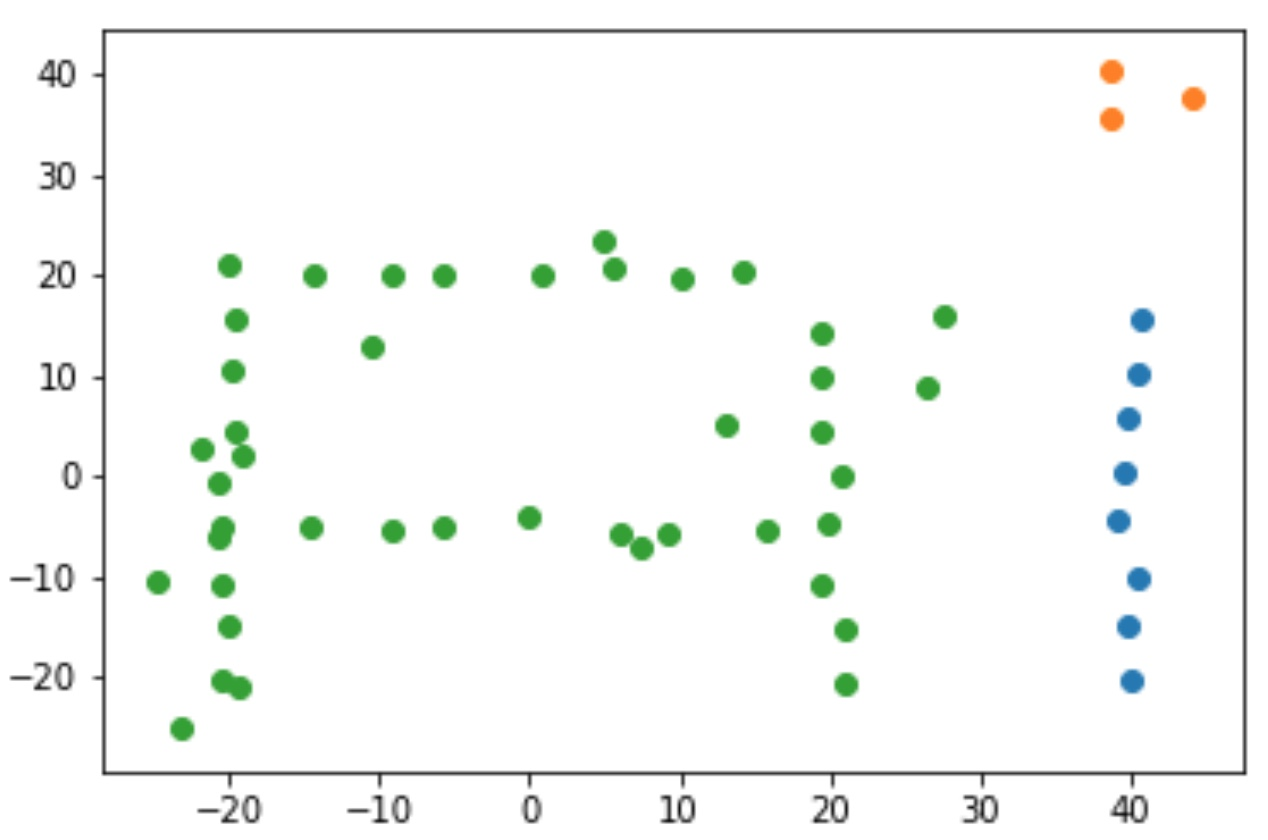
\includegraphics[scale=0.2]{ec_plot}
\end{center}

I'm inferring that the above plot is a reference to the AI Magazine. This is the link to the Table of Contents of the most recent issue(Volume 38, Number 3).

The author of the first article "Steps Toward Robust Artificial Intelligence" is "Thomas G. Dietterich". He is  Emeritus Professor of computer science at Oregon State University. \\

\underline{Interesting facts}
\begin{itemize}
	\item Thomas G. Dietterich has 347 publications to his credit on Google Scholar.
	\item From 2014-2016, he was the President of the Association for the Advancement of Artificial Intelligence(AAAI)
	\item As a PhD student, he sang in the Stanford University Chorus. It was in the choir that he met Carol Rivin, who would later become his wife
\end{itemize}
\newpage
\end{document}




























